\enquote{To a computer, the Web is a flat, boring world, devoid of meaning. This is a pity, as in fact documents on the Web describe real objects and imaginary concepts, and give particular relationships between them. For example, a document might describe a person. The title document to a house describes a house and also the ownership relation with a person. Adding semantics to the Web involves two things: allowing documents which have information in machine-readable forms, and allowing links to be created with relationship values. Only when we have this extra level of semantics will we be able to use computer power to help us exploit the information to a greater extent than our own reading.} - \textit{Tim Berners-Lee "W3 future directions" keynote, 1st World Wide Web Conference Geneva, May 1994} \cite{tim}

Revenons en au web sémantique afin de clarifier quelques termes et approfondir son mode de fonctionnement. Cela nous permettra de mieux comprendre tous les outils liés à la sémantique comme les knowledge graph. Actuellement la navigation et la recherche d'information sur le web nécessitent une action humaine. Une machine n'est pas encore capable de rechercher et d'analyser efficacement des données sur le web. La collecte de données automatique est possible mais la machine ne peut déterminer de manière fiable le type d'entité, les thèmes, les relations, le contexte, etc... des données qu'elle manipule.
\\*
Les aspirations du W3C sont de créer un web exploitable par des machines en le transformant en une base de connaissance géante.
La navigation sur le web est possible via des hyperliens, cependant elle doit aussi pouvoir se faire au niveau de données structurées pour que les machines puissent exploiter de façon plus efficiente et précise les données contenues sur le web.

Le web sémantique ou web 3.0 est une extension du web, standardisée par le W3C. Ces standards recommandent l'utilisation de format de données et de protocoles normés, plus généralement il s'agit du RDF (Resource Description Framework).

\subsubsection{RDF}

Le RDF (Ressource Description Framework) est un modèle de description des données permettant l'échange entre différentes applications. Il permet la structuration, l'indexation et la standardisation des données disponibles sur le web. Un schéma simple est utilisé pour structurer les échanges et les relations entre les ressources (documents, personnes, concepts abstraits...). Sachant qu'une ressource est représentée par une IRI (International Resource Identifier), par définition unique, il est possible de lier différentes ressources entre elles en utilisant un triplet : <Subject, Property, Object> ou Subject et Object sont définis par des IRI. La propriété d'une relation spécifie la nature du lien entre les 2 ressources : isChildOf, diedIn... Pour spécifier ces relations, le RDF utilise le langage XML (ou RDF/XML) \cite{rdf}. C'est ce qu'on appel des données liées au linked-data.

Ainsi le web sémantique ressemble à un graphe géant regroupant plusieurs milliards de liens (triplets) permettant une navigation et une interrogation des données plus efficaces. En respectant le RDF, une entreprise, une université ou n'importe quelle entité peut ouvrir ses données au web afin qu'elles soient exploitables par n'importe quelle machine.

Le RDF permet l'utilisation de différents "vocabulaires" ou ontologie pour traiter les données. Il pourrait être comparé à une grammaire et une ontologie à son vocabulaire. Par exemple FOAF (Friend Of A Friend) est une ontologie permettant la structuration de personnes. \cite{foaf}

\subsubsection{Ontologie}

Une ontologie permet de représenter les connaissances en les organisant sous forme de classes, de relations, de règles (ou implication) etc... Le but ici est de structurer les informations collectées sur le web.

Une ontologie se structure en essayant de comprendre le monde : comment est structuré notre monde, par quels concepts est-il défini ? Quelles sont les relations entre ces concepts permettant d'expliquer notre monde. Une ontologie ne s'intéresse donc par à ce qui est possible ou ce qui pourrait être mais s'intéresse à ce qui est. \cite{shirky} \cite{schema}

Toutes ces règles, conventions, standards et vocabulaires ont pour objectif de normaliser l'échange de données liées au web afin de construire un web dans lequel les ressources sont identifiables non par des urls mais par des données. Ainsi deux sources de données différentes qui utilisent les mêmes ontologies peuvent fusionner sans problèmes, et l'interrogation distincte de ces sources se fait avec les mêmes requêtes.

Par exemple, comme dans la figure \ref{fig1}, et via The Open Graph protocol (OGP) il est possible d'intégrer des balises HTML qui vont ajouter de la sémantique à un objet \cite{ogp}. Cela permet de rendre cet objet interopérable. Il pourra être ensuite traité de façon complexe avec d'autres objets.

\begin{figure}[ht]
\centering
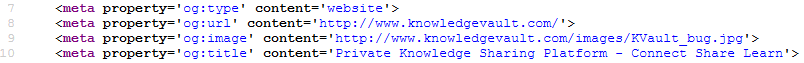
\includegraphics[width=\textwidth, draft=false]{imgs/og_example.PNG}
\caption{Exemple d'utilisation de l'open graph dans le code source d'une page : \url{http://www.knowledgevault.com/}}
\label{fig1}
\end{figure}

Ces données peuvent ensuite être collectées pour être rassemblées et raffinées dans des bases de connaissance telles que Yago.

\subsubsection{Exemple : Yago}

Une KB (knowledge base ou base de connaissance) est une base de données utilisée pour stocker et structurer du contenu lié à un domaine spécifique afin qu'il soit exploitable par une machine. Une KB lie ses données entre elles en y appliquant des règles, des faits ou des prédicats. A partir de ces constats, la KB peut déduire et faire évoluer la structuration de ses données. Prenons un exemple simple, j'ai une ontologie qui décrit les relations entre les personnes. En particulier cette ontologie me dit que si 2 personnes ont une même mère alors elles ont une relation fraternelle. Ainsi si j'enregistre 1 personne, ici la mère, et que je lui attribue un lien de maternité avec deux autres personnes, ma base sera capable de créer automatiquement un lien de fraternité entre ces 2 personnes.

Certaines KB ont pour but d'exploiter les données du web sémantique, la plupart se cantonne néanmoins, pour le moment, à la structuration des données présentes sur des domaines spécifiques, notamment wikipédia. On peut citer par exemple \href{http://wiki.dbpedia.org/about}{DBpedia} ou \href{https://www.wikidata.org/wiki/Wikidata:Main_Page}{Wikidata}, ou d'autres encore qui tentent d'étendre leur champ d'action à d'autres sources comme \href{http://www.mpi-inf.mpg.de/departments/databases-and-information-systems/research/yago-naga/yago/}{Yago}.

Yago est une KB créée par l'institut Max-Planck d'informatique à Sarrebrück en 2008. Contrairement à DBpedia ou Wikidata qui s'appuient sur un effort communautaire, le but de Yago est d'extraire des données de sources différentes (actuellement Wikipedia et Wordnet). Tout cela automatiquement et en plusieurs langues. Beaucoup de KB comme Yago s'organise sous la forme de graphe. L'information dans ces bases est représentées par un graphe géant constitué de millions de triples. Ces graphes sont appelés graphes de connaissance.

Les KB comme Yago permettent d'interroger Wikipedia et différentes sources avec des requêtes précises, par exemple : "Les peintres français du 16ème siècle" ou "Les villes de Chine de plus d'un million d'habitants". Les requêtes après traitement se font en langage naturel et retourne des données structurée et formatée pour être utilisée directement avec le système. Yago regroupe actuellement des informations sur plus de 10 millions d'entité (personnes, villes, etc.) et plus de 120 millions de faits sur ces entités. 
Il existe de nombreuses bases de connaissances qui contiennent des données hétérogènes comme Yago mais d'autres se concentrent sur des domaines spécifiques comme la médecine (ex : Precision Medicine Knowledgebase). Ces bases apportent une matière essentiel à la lutte contre la désinformation, ce sont des sources de données fiables et dont le requêtage est facilement automatisable.
Le langage d'interrogation de ces données est le SPARQL.

Yago est disponible en open source \href{https://github.com/yago-naga/yago3}{ici}.

\iffalse
\subsubsection{SPARQL}

SPARQL (Protocol And RDF Query Language) est un langage de requête orienté données permettant d'intéragir avec des données RDF à travers le web. SPARQL permet de questionner le web sémantique, plus précisément les triplets, qui forme le graphe géant du web sémantique.

Exemples pour Yago (n'est plus accessible sur les SPARQL endpoints donc non testable pour le moment) :

Liste des prédicats associés à l'entité France.

\begin{lstlisting}[language=SPARQL, backgroundcolor=\color{lightgray}]
PREFIX rdf: <http://www.w3.org/1999/02/22-rdf-syntax-ns#> 
PREFIX yago: <http://yago-knowledge.org/resource/>
SELECT DISTINCT ?x WHERE {
    yago:France rdf:type ?x.
}
\end{lstlisting}

\iffalse
Savoir si l'entité France est référencée sur wikipedia.

\begin{lstlisting}[language=SPARQL, backgroundcolor=\color{lightgray}]
PREFIX rdf: <http://www.w3.org/1999/02/22-rdf-syntax-ns#> 
PREFIX yago: <http://yago-knowledge.org/resource/>
SELECT DISTINCT ?x WHERE {
    yago:France yago:hasWikipediaUrl ?x.
}
\end{lstlisting}

\fi

Autre exemple sur DBPedia, dans quelles catégories s'inscrit une voiture ?

\begin{lstlisting}[language=SPARQL, backgroundcolor=\color{lightgray}]
PREFIX dbr: <http://dbpedia.org/resource/>
PREFIX  dct:  <http://purl.org/dc/terms/> 

select ?categorie, (COUNT(?result) as ?numberResult) 
where {
   ?result dct:subject ?categorie.
   ?search rdfs:label "Voiture"@fr .
   ?search <http://dbpedia.org/ontology/wikiPageWikiLink> 
   ?categorie
} ORDER BY ?numberResult
LIMIT 1000
\end{lstlisting}

Tester \href{http://fr.dbpedia.org/sparql?default-graph-uri=&query=PREFIX+dbr\%3A+\%3Chttp\%3A\%2F\%2Fdbpedia.org\%2Fresource\%2F\%3E\%0D\%0APREFIX++dct\%3A++\%3Chttp\%3A\%2F\%2Fpurl.org\%2Fdc\%2Fterms\%2F\%3E+\%0D\%0A\%0D\%0Aselect+\%3Fcategorie\%2C+\%28COUNT\%28\%3Fresult\%29+as+\%3FnumberResult\%29+\%0D\%0Awhere+\%7B\%0D\%0A+++\%3Fresult+dct\%3Asubject+\%3Fcategorie.\%0D\%0A+++\%3Fsearch+rdfs\%3Alabel+\%22Voiture\%22\%40fr+.\%0D\%0A+++\%3Fsearch+\%3Chttp\%3A\%2F\%2Fdbpedia.org\%2Fontology\%2FwikiPageWikiLink\%3E+\%0D\%0A+++\%3Fcategorie\%0D\%0A\%7D+ORDER+BY+\%3FnumberResult\%0D\%0ALIMIT+1000&format=text\%2Fhtml&timeout=0&debug=on}{ici}

\subsubsection{Wikidata}

\todo{A mettre en forme et à intégrer sur un eexemple de fact checking}

Info : dans une entrée, si ns = 14, alors c'est une sous catégorie de l'objet recherché. Ici les requêtes sont limitées à 10 résultats.

Faire une recherche : 

\url{https://fr.wikipedia.org/w/api.php?action=query&list=search&format=jsonfm&srsearch=Panneau+solaire&utf8=1}

Rechercher une catégorie :

\url{https://fr.wikipedia.org/w/api.php?action=query&titles=Panneau+solaire&prop=categories&clshow=hidden&utf8=1}

clshow=hidden permet d'afficher les catégories cachées comme les portails qui sont bien plus génériques que les catégories.

clshow=!hidden permet de n'afficher que les catégories spécifiques de l'article, la recherche est bien plus simple.

Catégories liées aux Technologies :

\url{https://fr.wikipedia.org/w/api.php?action=query&list=categorymembers&cmtitle=Category:Technologie&utf8=1}

Catégories principales de wikipédia (portails, en anglais)

\url{https://en.wikipedia.org/w/api.php?action=query&list=categorymembers&cmtitle=Category:Main%20topic%20classifications&utf8=1}

Plus d'infos : 

\url{https://www.mediawiki.org/wiki/API:Categories}

\url{https://m.mediawiki.org/wiki/API:Query#Generators}
\fi

\subsubsection{Conclusion}

Le web sémantique est une source de données interopérable qui traite des données complexes. La donnée représente un objet, cet objet a des relations, des attributs et des propriétés. Mis bout à bout ces objets permettent d'avoir une représentation concrète de la réalité dans un ou plusieurs domaines. C'est cet ancrage dans la réalité qui donne au web sémantique le contexte qui manque aux données brutes. Les données liées sont primordiales pour faire évoluer le fact checking vers des approches plus performantes et fiables.